\documentclass[11pt,a4paper]{article}

\usepackage[utf8]{inputenc} 
\usepackage[T1]{fontenc} 
\usepackage{lmodern}
\usepackage[margin=2cm]{geometry}
\usepackage[german]{babel}
\usepackage{amsmath} 
\usepackage{graphicx} 
\usepackage{cancel}
\usepackage{booktabs}
\usepackage{hyperref}
\usepackage{tikz}
\hypersetup{
    colorlinks,
    citecolor=red,
    filecolor=black,
    linkcolor=black!20!blue!90!,
    urlcolor=black} 
\usepackage{nicefrac}
%\usepackage[table]{xcolor}
\usepackage{tocloft}

\setlength{\parindent}{0pt}
\setlength{\parskip}{1ex plus 0.5ex minus 0.5ex}

\definecolor{incolor}{rgb}{0.0, 0.0, 0.5}

\hbadness=99999

\newcommand{\refpy}[1]{Siehe Anhang: \textit{Rechnungen in Python} (\texttt{{\color{incolor}In [{\color{incolor}#1}]}})}
\newcommand\dif{\mathop{}\!\mathrm{d}}
\newcommand{\halftime}[4]{\begin{figure}[h]
\begin{minipage}{.#1\textwidth}#3\end{minipage}\begin{minipage}{.#2\textwidth}
\centering
#4\end{minipage}
\end{figure}}
\renewcommand{\vec}{\boldsymbol}
\newcommand\mean{\begin{equation}
\bar{x}=\frac{\sum_{i=1}^n x_{i}}{n}\label{mean}
\end{equation}}
\newcommand\meanstd{\begin{equation}
s_{\bar{x}}=\frac{s_x}{\sqrt{n}}\label{meanstd}
\end{equation}}
\newcommand\prodquo{\begin{equation}\left\vert\frac{\Delta z}{z}\right\vert=\sqrt{\left(a\frac{\Delta x}{x}\right)^2+\left(b\frac{\Delta y}{y}\right)^2+\ldots}\textrm{ f\"ur }z=x^a\ y^b\ldots\end{equation}}
\newcommand\tfunc{\begin{equation}
\frac{\vert x-y_0\vert}{u_x}
\end{equation}}

\begin{document}

% name of experiment
% date of experiment
% name of assistant
{
\centering 
\large 
Physiklabor für Anf\"anger*innen \\
Ferienpraktikum im Sommersemester 2018 \\[4mm]
\textbf{\LARGE 
Versuch 70: Linsen und Linsensysteme
} \\[3mm]
(durchgef\"uhrt am 28.09.2018 bei Daniel Bartel) \\
Andréz Gockel, Patrick M\"unnich\\
\today \\[10mm]
}

\vspace{50pt}
\tableofcontents
\vspace{22pt}
\listoftables
\vspace{22pt}
\listoffigures
\pagebreak

\section{Ziel des Versuchs}

Das Ziel dieses Versuchs ist es, Einzellinsen und Linsenkombinationen zu untersuchen. Genauer schaut man, wann mit welchen Linsen scharfe Abbildungen von Gegenst\"anden vorhanden sind.

\section{Teil 1}

\subsection{Theorie}

F\"ur das Verst\"andnis dieses Teils ben\"otigt man die Abbildungsgleichung f\"ur d\"unne Linsen,
\begin{equation}
\frac{1}{f}=\frac{1}{g}+\frac{1}{b},\label{eq:1}
\end{equation}

und die entsprechende Gleichung f\"ur Linsensysteme mit zwei Linsen,
\begin{equation}
\frac{1}{f}=\frac{1}{f_1}+\frac{1}{f_2}-\frac{d}{f_1f_2}.\label{eq:2}
\end{equation}

Dieses l\"asst sich f\"ur kleine Abst\"ande $d$ zwischen den Linsen zu
\[
\frac{1}{f}\approx\frac{1}{f_1}+\frac{1}{f_2}
\]
vereinfachen.


\subsection{Aufbau}

% describe set up
% insert pic name, designation, toc caption, caption, label

%\halftime{5}{5}{TEXT}{\fbox{\includegraphics[width=0.5\textwidth]{NAME}}
%   \renewcommand\thefigure{BX}
%\caption[XXXX]{XXXX \cite{Anleitung}}
%\label{Pic:X}}

\subsection{Durchführung}

% describe exp.
XXXX

\subsection{Auswertung}

In diesem Teil wollen wir einfach $\nicefrac{1}{b}$ gegen $\nicefrac{1}{g}$ auftragen. Die gesch\"atzten Fehler werden als Fehlerbalken eingezeichnet. Zum Vergleich werden noch Geraden addiert, welche f\"ur die Linse mit $f=80\,$mm mit
\[
\frac{g}{f}
\]
berechnet wurde und f\"ur die Linsensysteme mit jeweils $f_1=80\,$mm und $f_2=150\,$mm bzw. $f_1=80\,$mm und $f_2=200\,$mm mit
\[
\frac{1}{f_1}+\frac{1}{f_2}-\frac{1}{g}
\]
bestimmt. Die resultierende Graphik kann im Anhang als Abbildung \ref{Abb:1} gefunden werden.

\section{Teil 2}

\subsection{Theorie}

F\"ur diesen Teil f\"uhren wir neue Variablen ein:
\begin{itemize}
\item Abstand $s=g+b$ zwischen Gegenstand und Bild
\item Differenz $e=|g-b|$ zwischen den Linsenpositionen.
\end{itemize}

Diese Variablen setzen wir in (\ref{eq:1}) ein und erhalten:

\[
\frac{1}{f}=\frac{2}{s+e}+\frac{2}{s-e}
\]
\[
=\frac{2s-\bcancel{2e}+2s+\bcancel{2e}}{s^2-e^2}
\]
\[=\frac{4s}{s^2-e^2}\]
\begin{equation}
f=\frac{s^2-e^2}{4s}\label{eq:3}
\end{equation}

\subsection{Aufbau}

% describe set up
% insert pic name, designation, toc caption, caption, label

%\halftime{5}{5}{TEXT}{\fbox{\includegraphics[width=0.5\textwidth]{NAME}}
%   \renewcommand\thefigure{BX}
%\caption[XXXX]{XXXX \cite{Anleitung}}
%\label{Pic:X}}

\subsection{Durchführung}

% describe exp.
XXXX

\subsection{Auswertung}

In diesem Teil wollen wir einfach mit unseren Messwerten und der Formel (\ref{eq:3}) zuerst unsere Werte f\"ur $(s,e)$:

\begin{table}[h]
\centering
\caption{XXXX} \vspace{11pt}
$\begin{array}{l}
\textrm{Unsicherheiten:}\\
\textrm{s: } \pm 0.4 \textrm{cm}\\
\textrm{e: } \pm 0.5 \textrm{cm}\\
\end{array}$
\begin{tabular}{ccc}
\toprule
\textrm{XXXX}/\textrm{XX} & \textrm{XXXX}/\textrm{XX} & \textrm{XXXX}/\textrm{XX} \\
\midrule 
2 & 0.26 & 0.23\\
\hline
4 & 0.33 & 0.25\\
\hline 
5 & & 0.3\\
\hline 
6 & 1.25 & 0.83\\
\hline 
8 & 3.9 & 0.83\\ 
\hline
9 & 4.75 & 4.6\\ 
\hline
10 & 4.7 &\\ 
\bottomrule
\end{tabular}
\phantom{$\begin{array}{l}
\textrm{Unsicherheiten:}\\
\textrm{s: } \pm 0.4 \textrm{cm}\\
\textrm{e: } \pm 0.5 \textrm{cm}\\
\end{array}$}
\label{Tab:X}
\end{table}

Wir k\"onnen hier die Rechnungen per Hand mit Gau\ss scher Fehlerfortpflanzung durchf\"uhren. Hierzu m\"ussen wir unsere Gleichung einfach nach jeweils $e$ und $s$ partiell ableiten:

\[
\frac{\partial f}{\partial s}=\frac{s^2+e^2}{4s}
\]
\[
\frac{\partial f}{\partial e}=\frac{-e}{2s}
\]

Dies k\"onnen wir in
\[
\Delta f=\sqrt{\left(\frac{\partial f}{\partial s}\Delta s\right)^2+\left(\frac{\partial f}{\partial e}\Delta e\right)^2}
\]
einsetzen und berechnen. In diesem Fall sind unsere Ergebnissen jedoch mit dem \textit{uncertainties} Paket in Python berechnet worden. \refpy{12} Dieses Paket hat die F\"ahigkeit, Korrelationen zwischen Variablen zu ber\"ucksichtigen \cite{Uncertainties}.

Da uns hier die Mittelwerte interessieren, nutzen wir noch

\mean

f\"ur die Berechnung des Mittelwerts und

\meanstd

f\"ur der Berechnung der Unsicherheit dessen.

Wir erhalten daraus f\"ur die Linse mit $f=80\,$mm $\bar{f}=82\pm1.7\,$mm, f\"ur das System mit $f_1=80\,$mm und $f_2=150\,$mm $\bar{f}=58\pm1.9\,$mm und f\"ur das Linsensystem mit $f_1=80\,$mm und $f_2=200\,$mm $\bar{f}=123\pm1.4\,$mm.

\section{Teil 3}

\subsection{Theorie}

F\"ur das Abbe-Verfahren f\"uhren wir den Abbildungsma\ss stab ein:
\begin{equation}
\beta=\frac{B}{G}=\frac{b}{g}\label{eq:4}
\end{equation}
Dies machen wir, da wir $b$ und $g$ nicht direkt bestimmen k\"onnen, jedoch die Bildgr\"o\ss e $B$ und Gegenstandsgr\"o\ss e $G$ problemlos bestimmen k\"onnen.

Die Hauptebenen befinden sich dann um $h_{1/2}$ vor bzw. hinter diesem Punkt. Mit unserer messbaren scheinbaren Gegenstandsgr\"o\ss e $g'$ und scheinbare Bildweite $b'$ haben wir also
\begin{equation}
g'=\left(1+\nicefrac{1}{\beta}\right)f_1+h_1\label{eq:5}
\end{equation}
\begin{equation}
b'=\left(1+\beta\right)f_2+h_2\label{eq:6}
\end{equation}

\subsection{Aufbau}

% describe set up
% insert pic name, designation, toc caption, caption, label

%\halftime{5}{5}{TEXT}{\fbox{\includegraphics[width=0.5\textwidth]{NAME}}
%   \renewcommand\thefigure{BX}
%\caption[XXXX]{XXXX \cite{Anleitung}}
%\label{Pic:X}}

\subsection{Durchführung}

% describe exp.
XXXX

\subsection{Auswertung}

In diesem Teil wollen wir zuerst mit den Formeln (\ref{eq:4}), (\ref{eq:5}) und (\ref{eq:6}) $g'$, $b'$, $\beta$ und $\Delta \beta$ bestimmen. Wir erhalten aus unseren Messreihen:

Um dies visuell darzustellen, tragen wir $1+\nicefrac{1}{\beta}$ gegen $g'$ und $1+\beta$ gegen $b'$ auf.

\begin{figure}[h]
\centering
\fbox{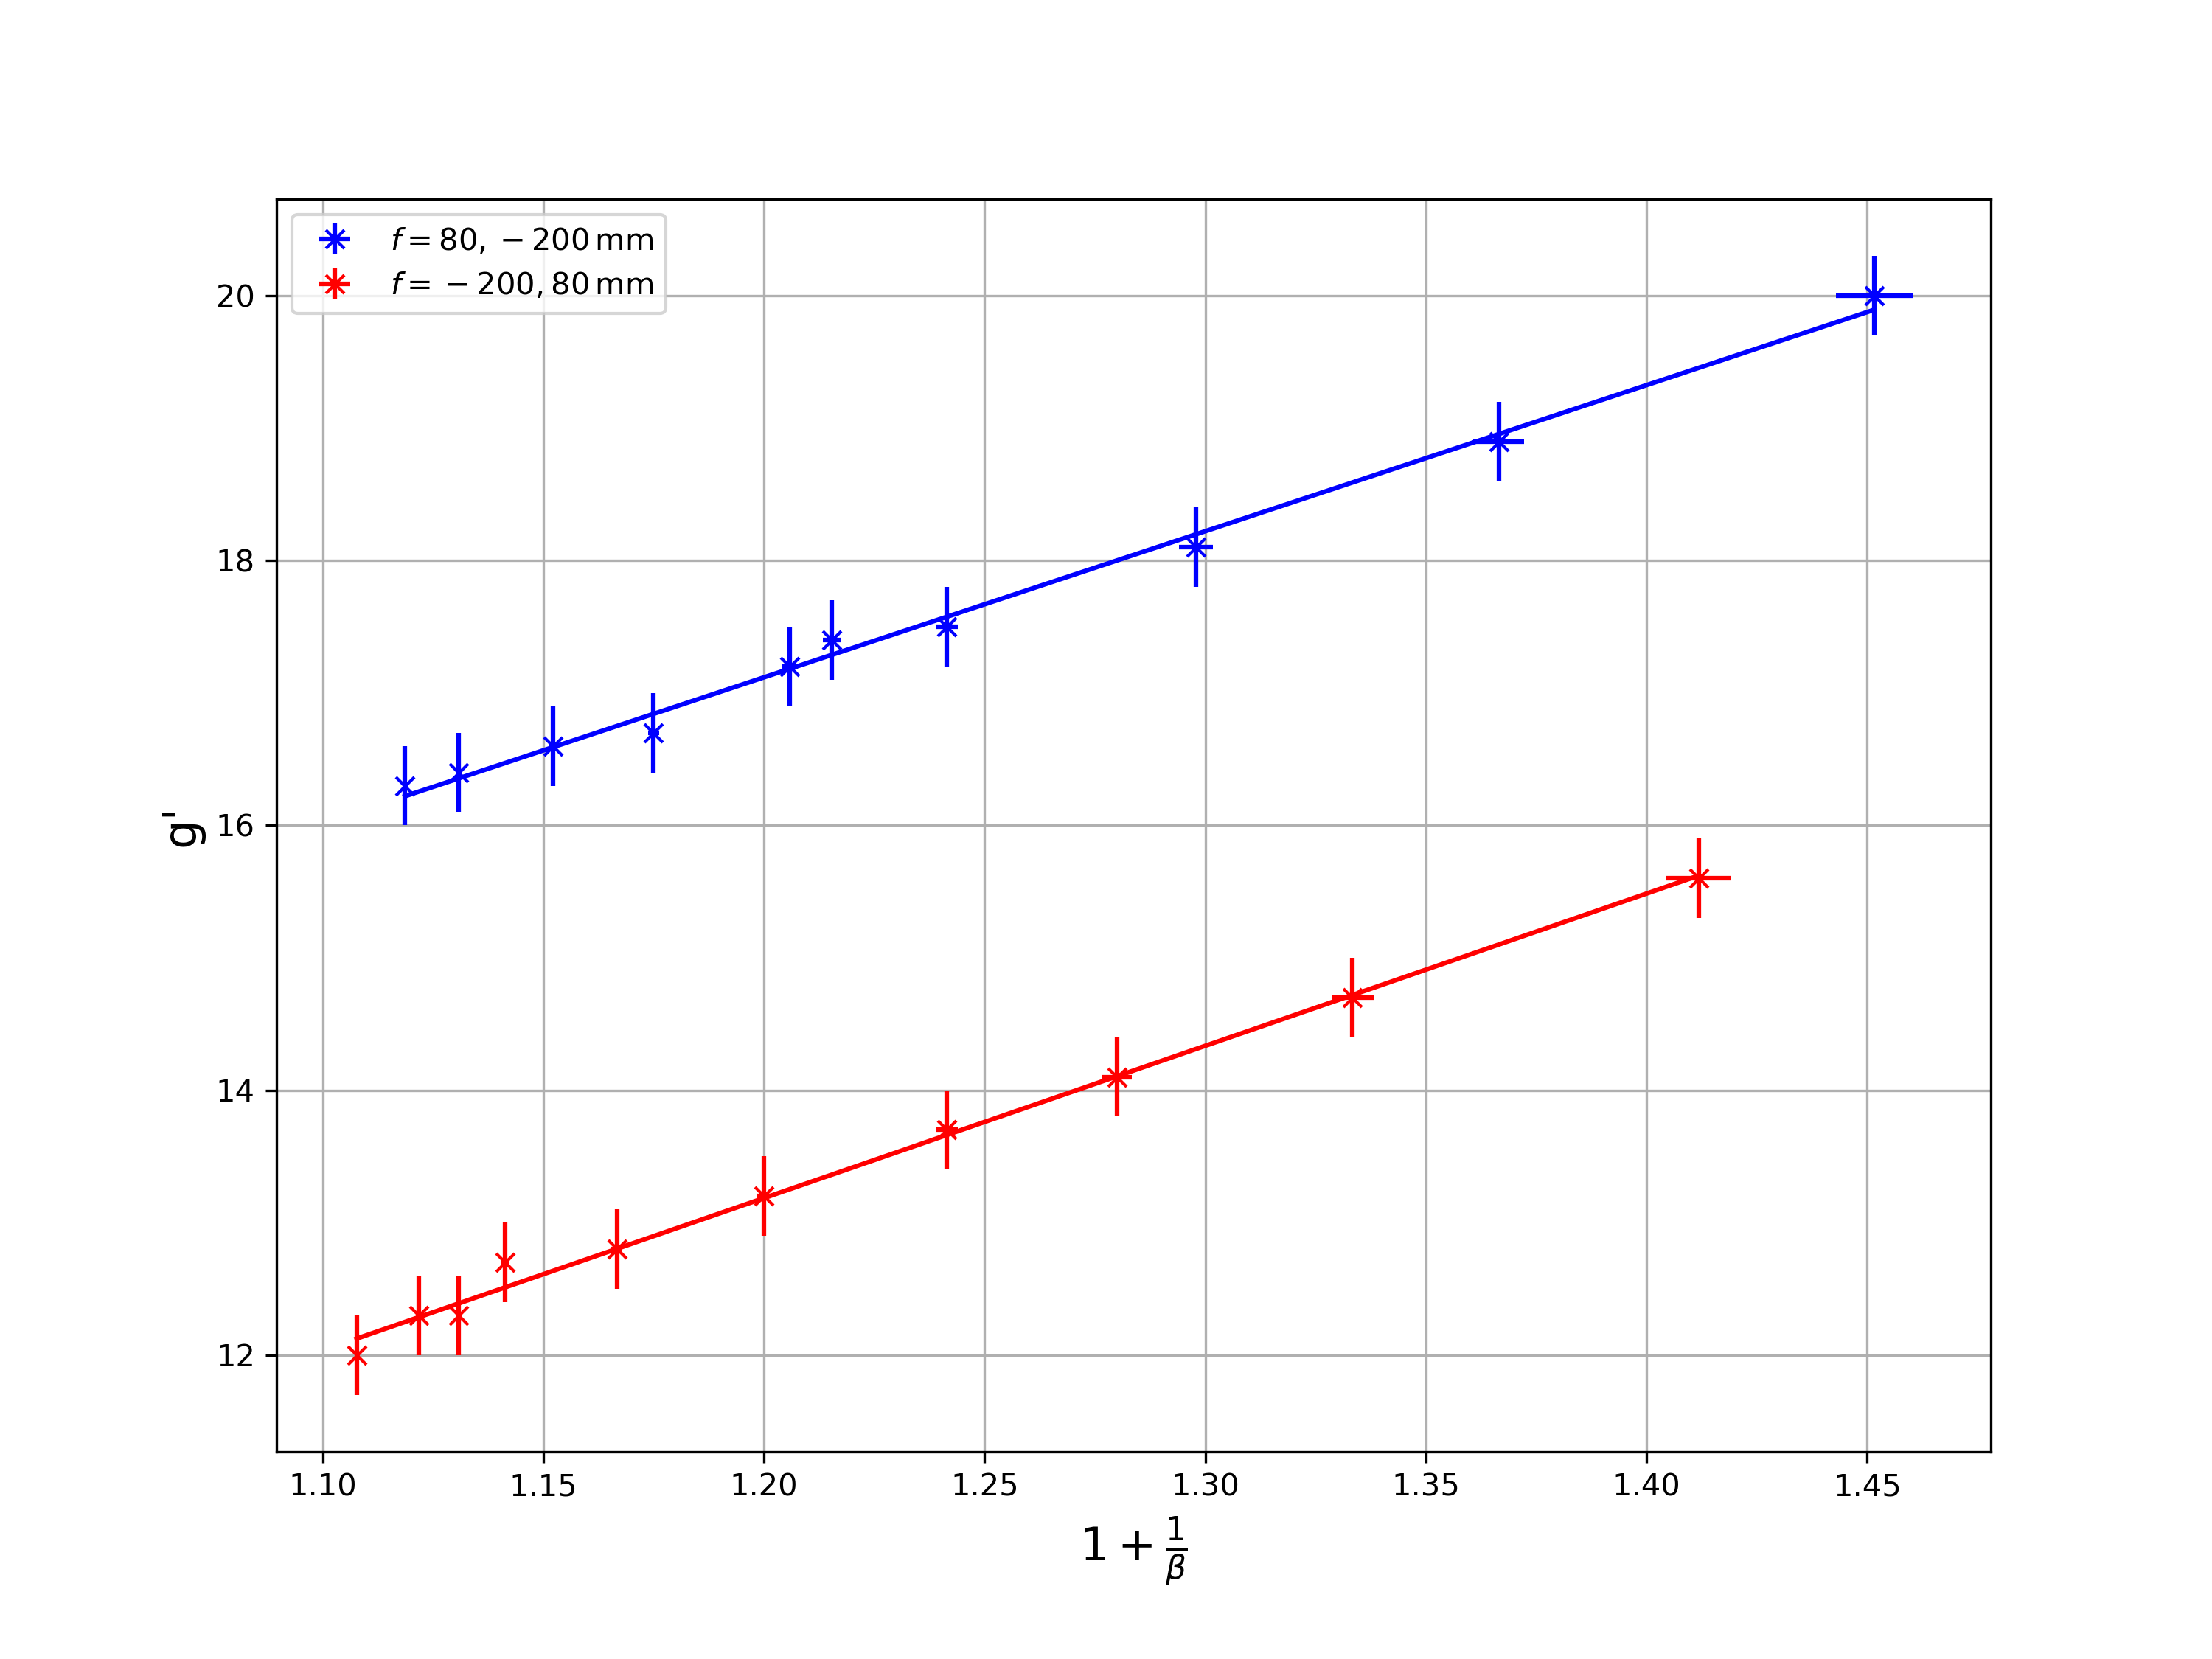
\includegraphics[width=0.8\textwidth]{g.png}}
\renewcommand\thefigure{69}
\caption[$1+\nicefrac{1}{\beta}$ gegen $g'$ dargestellt]{$1+\nicefrac{1}{\beta}$ gegen $g'$ dargestellt}
\label{Abb:g}
\end{figure}

\begin{figure}[h]
\centering
\fbox{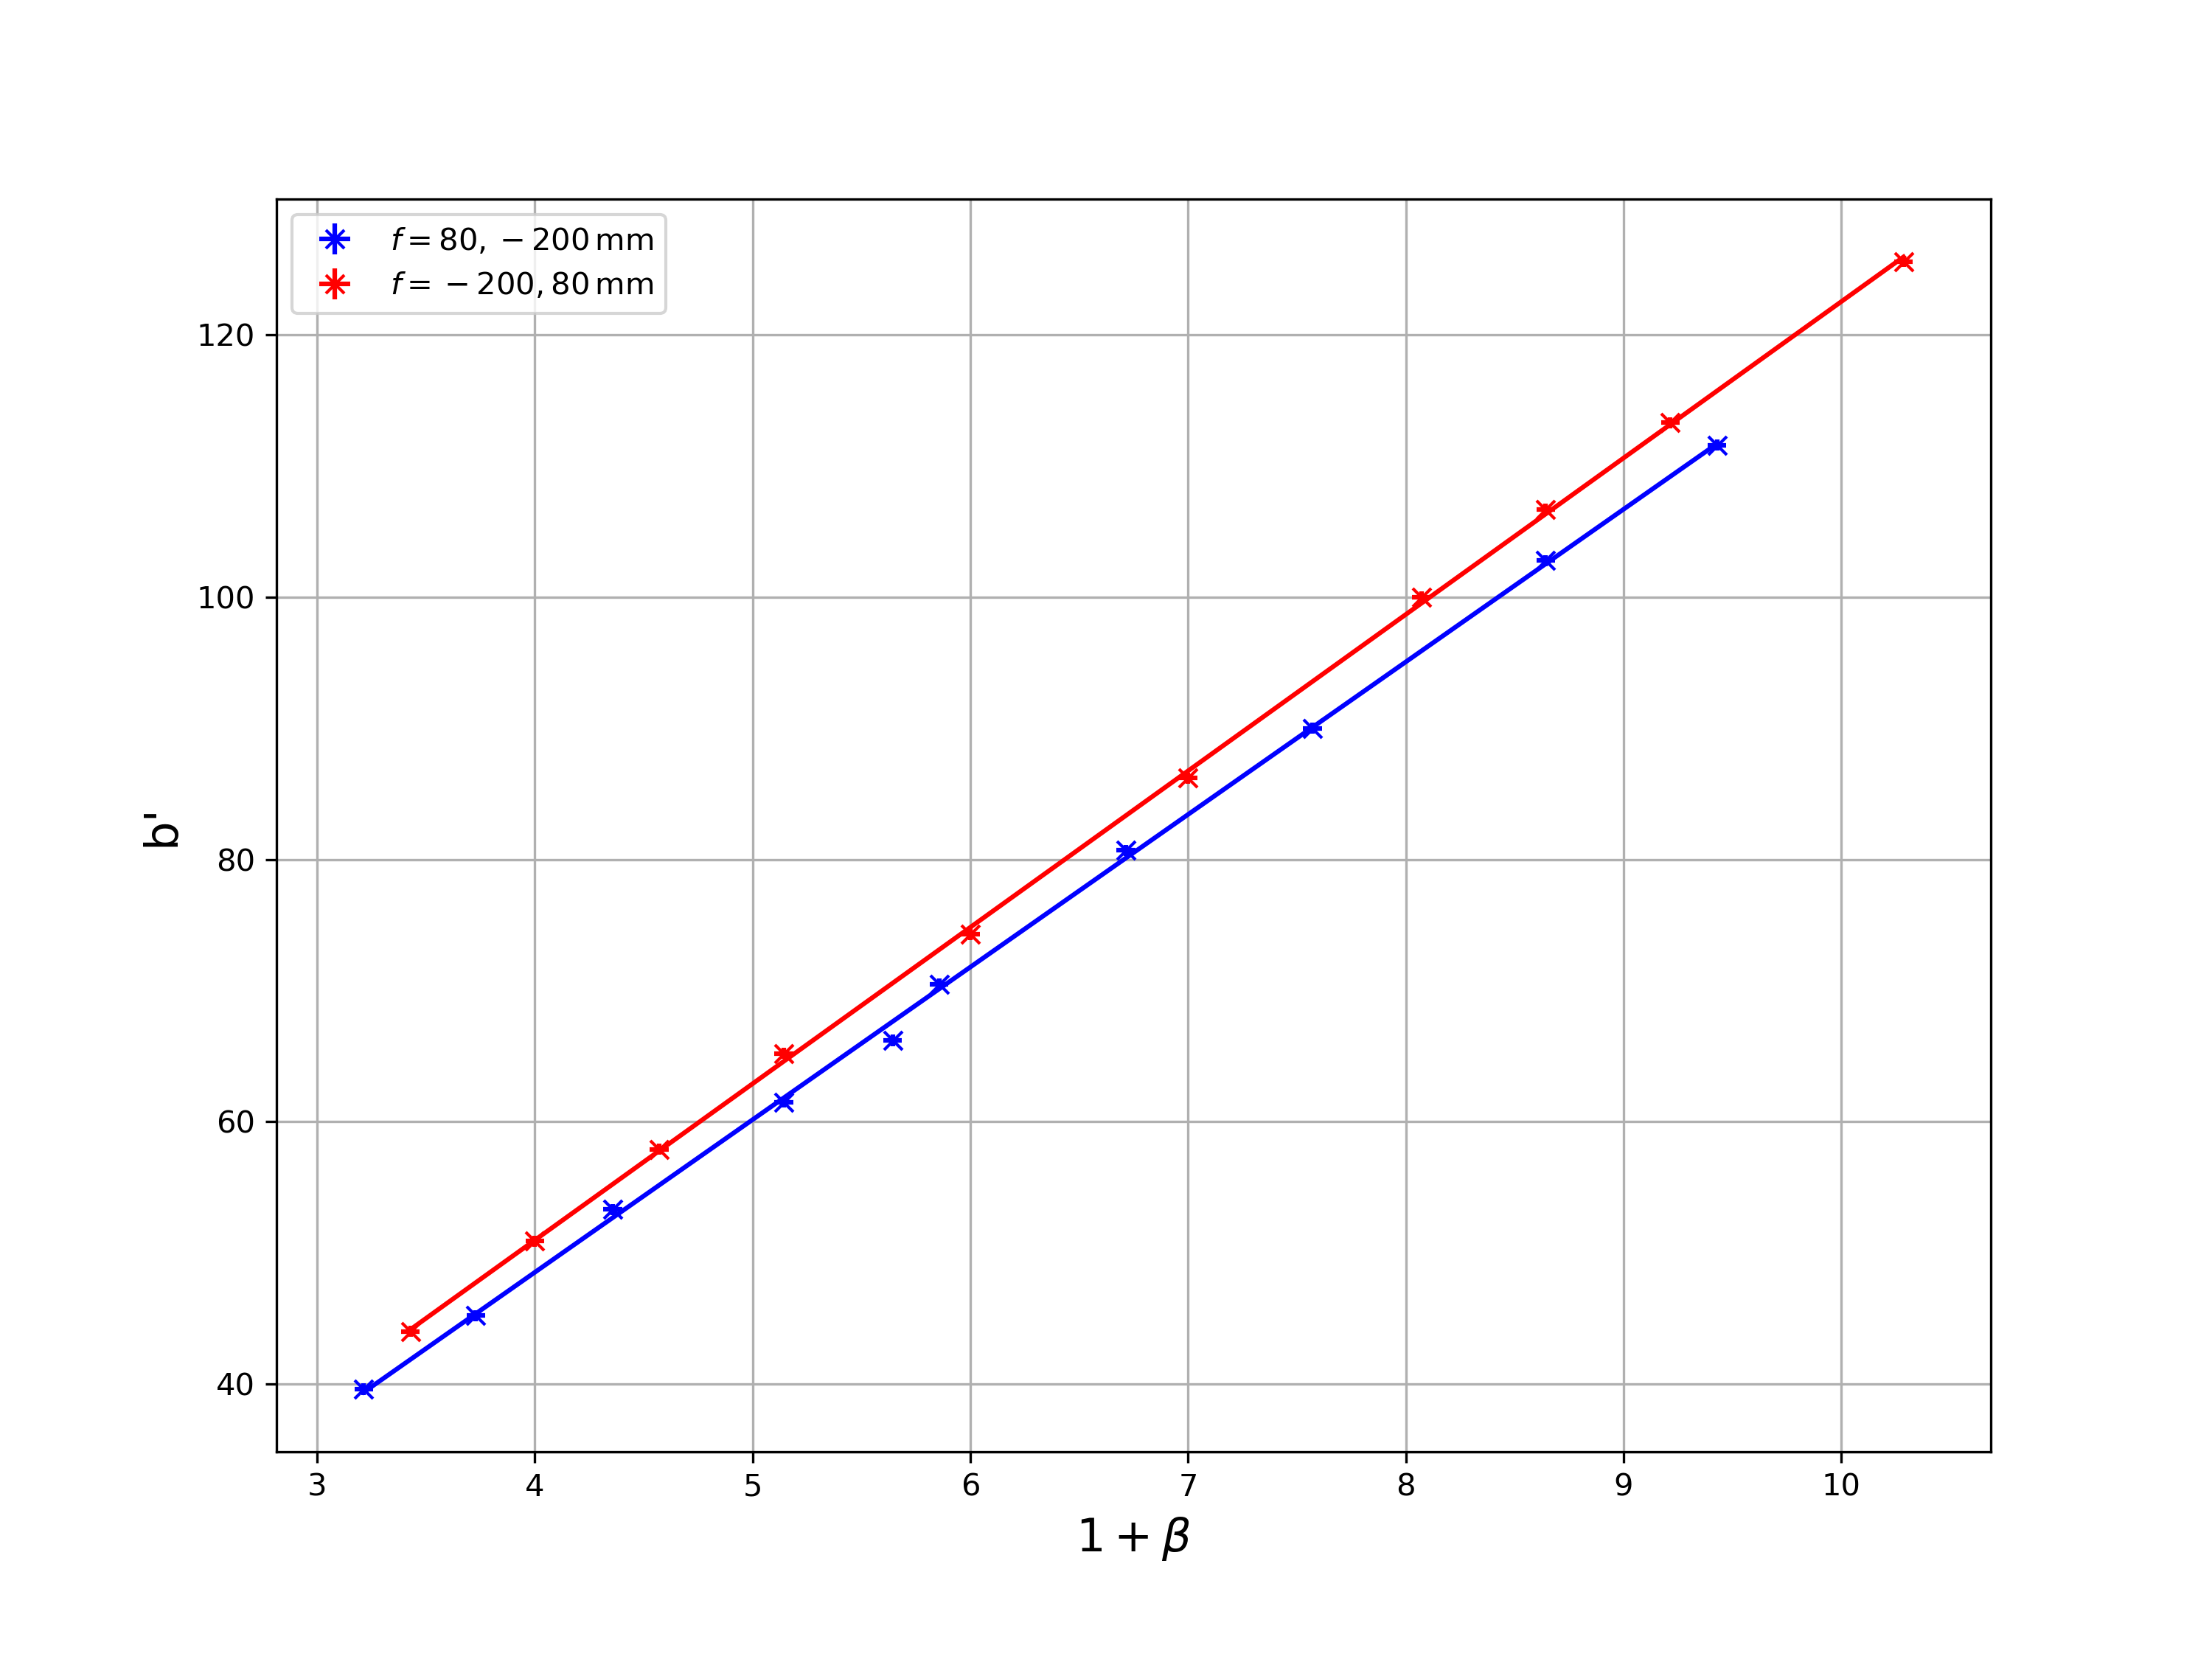
\includegraphics[width=0.8\textwidth]{b.png}}
\renewcommand\thefigure{420}
\caption[$1+{\beta}$ gegen $b'$ dargestellt]{$1+\beta$ gegen $b'$ dargestellt}
\label{Abb:b}
\end{figure}

Aus der linearen Regression k\"onnen wir $f_1$, $f_2$, $h_1$ und $h_2$ bestimmen. 

Zur Bestimmung der linearen Regression wenden folgende Formeln an:

\begin{equation}
a=\frac{n\sum x_iy_i-\sum x_i\sum y_i}{n\sum x_i^2-(\sum x_i)^2}
\end{equation}
\begin{equation}
\Delta a=s\sqrt{\frac{n}{n\sum x_i^2-(\sum x_i)^2}},
\end{equation}
\begin{equation}
b=\frac{\sum x_i^2\sum y_i-\sum x_i\sum x_iy_i}{n\sum x_i^2-(\sum x_i)^2}
\end{equation}
\begin{equation}
\Delta b=s\sqrt{\frac{\sum x_i^2}{n\sum x_i^2-(\sum x_i)^2}}
\end{equation}
\begin{equation}
s=\sqrt{\frac{1}{n-2}\sum^n_{i=1}[y_i-(a+bx_i)]^2},
\end{equation}

Wir erhalten als Werte:

\begin{table}[h]
\centering
\caption{XXXX} \vspace{11pt}
$\begin{array}{l}
\textrm{Unsicherheiten:}\\
\textrm{XXXX: } \pm XX \textrm{XX}\\
\end{array}$
\begin{tabular}{cccc}
\toprule
\textrm{XXXX}/\textrm{XX} & \textrm{XXXX}/\textrm{XX} & \textrm{XXXX}/\textrm{XX} \\
\midrule 
$f_1$ & 80 & -200 & 0.5762491658548258\\
$h_1$ & 80 & -200 & 11.03475419102985\\
$f_2$ & 80 & -200 & 1.9531933609241\\
$h_2$ & 80 & -200 & 11.639603091057374\\
$f_1$ & -200 & 80 & -3.913845161813182\\
$h_1$ & -200 & 80 & 11.49900273595246\\
$f_2$ & -200 & 80 & 3.2411227934990583\\
$h_2$ & -200 & 80 & 11.930724229182056\\
\bottomrule
\end{tabular}
\phantom{$\begin{array}{l}
\textrm{Unsicherheiten:}\\
\textrm{XXXX: } \pm XX \textrm{XX}\\
\end{array}$}
\label{Tab:X}
\end{table}


Zur Klarifizierung fertigen wir noch eine (au\ss er der Linsen) ma\ss stabsgetreue Skizze an:\\
\\
\begin{figure}
\begin{center}
\begin{tikzpicture}[scale=0.6]%, inner sep=0]
\def\sx{0.3}

% Optische Achse
\draw[dashed, thick] (-30*\sx,0) -- (50*\sx,0);
% Koordinaten Nullpunkt
\draw (0,-0.2) -- (0,0.2);

% Konkave Linse
\def\xconv{0.5} % x-Koordinate
\draw[thick, fill=yellow!30] 
     ([shift=(190:16cm)]16.5+\xconv,0) arc (190:170:16cm)
     -- ([shift=(10:16cm)] -16.5+\xconv,0)
     arc (10:-10:16cm) 
     -- ([shift=(190:16cm)]16.5+\xconv,0);

% Konvexe Linse
\def\xconx{-1.5} % x-Koordinate
\draw[thick, fill=yellow!30] ([shift=(-15:10cm)]-9+\xconx,0) arc (-15:15:10cm)
 --([shift=(165:10cm)]10+\xconx,0) arc (165:195:10cm)
 --([shift=(-15:10cm)]-9+\xconx,0);

% Gegenstand (Pfeil)
\def\Gx{-20.0*\sx}
\def\Gy{0.7}
\node [inner sep=0] (G) at (\Gx,\Gy) {};
\draw[->, ultra thick, left] (\Gx,0) to node {\tiny $7\,$mm} (G);%
\node (labG) at (\Gx,\Gy+0.5) {$G$};
% Bild (arrow)
\def\Bx{39.6*\sx}
\def\By{-1.55}
\node[inner sep=0] (B) at (\Bx,\By) {};
\draw[->, ultra thick, right] (\Bx,0) to node {\tiny $17\,$mm}  (B);
\node (labB) at (\Bx,\By-0.5) {$B$};

% Hauptebenen
\def\Hx{-3.9*\sx}
\def\Hxii{2.0*\sx}
\draw (\Hx,-4) -- (\Hx,4); % H1
\node (labH1) at (\Hx,4.5) {$H_1$};
\draw (\Hxii,-4) -- (\Hxii,4); % H2
\node (labH2) at (\Hxii,4.5) {$H_2$};

% Strahlen
% FokusG
\fill[blue] (\Hx,\By) circle [radius=0.1];
\fill[blue] (\Hxii,\By) circle [radius=0.1];
\fill[blue] (\Hx,0) circle [radius=0.1];
\fill[blue] (\Hx,\Gy) circle [radius=0.1];
\fill[blue] (\Hxii,\Gy) circle [radius=0.1];
\fill[blue] (\Hxii,0) circle [radius=0.1];
\draw[thick, color=blue] (G) -- (\Hx,\By);
\draw[thick, color=blue] (B) -- (\Hx,\By);
% FokusB
\draw[thick, color=blue] (G) -- (\Hxii,\Gy);
\draw[thick, color=blue] (B) -- (\Hxii,\Gy);
%Central
\draw[thick, color=blue] (G) -- (\Hx,0) -- (\Hxii,0)  -- (B);
               
% Label
%Fokus Punkte
\def\fxi{-11*\sx+\Hx}
\def\fxii{11.6*\sx+\Hxii}
\draw[red] (\fxi,-0.4) -- (\fxi,0.4);
\draw[red] (\fxii,-0.4) -- (\fxii,0.4);
\fill[red] (\fxi,0) circle [radius=0.1];
\fill[red] (\fxii,0) circle [radius=0.1];
\node (F1) at (\fxi,-0.8) {$F_1$};
\node (F2) at (\fxii,0.8) {$F_2$};
% Distanzen
\node (f1) at (\fxi,-3.5) {} ;
\node (h1) at (\Hx,-3.5) {} ;
\node (f2) at (\fxii,-3.5) {} ;
\node (h2) at (\Hxii,-3.5) {} ;
\draw[<->, below] (f1) to node {\tiny $f_1=11\,$cm} (h1) ;
\draw[<->, below] (f2) to node {\tiny $f_2=11.6\,$cm} (h2) ;
\draw[<->, below]%, inner sep=10] 
(h1) to node {\tiny $5.9\,$cm} (h2);

\node (g) at (\Gx,3.5) {} ;
\node (gh1) at (\Hx,3.5) {} ;
\node (b) at (\Bx,3.5) {} ;
\node (bh2) at (\Hxii,3.5) {} ;
\draw[<->, above] (g) to node {\small $g=20\,$cm} (gh1) ;
\draw[<->, above] (b) to node {\small $b=39.6\,$cm} (bh2) ;

% Koordinaten Nullpunkt
% x-Achse
\def\cy{-5}
\draw[->] (-30*\sx,\cy) -- (50*\sx,\cy);
\draw (0,-0.2+\cy) -- (0,0.2+\cy);
\draw (10*\sx,-0.2+\cy) -- (10*\sx,0.2+\cy);
\draw (-10*\sx,-0.2+\cy) -- (-10*\sx,0.2+\cy);
\draw (20*\sx,-0.2+\cy) -- (20*\sx,0.2+\cy);
\draw (-20*\sx,-0.2+\cy) -- (-20*\sx,0.2+\cy);
\draw (30*\sx,-0.2+\cy) -- (30*\sx,0.2+\cy);
\draw (-30*\sx,-0.2+\cy) -- (-30*\sx,0.2+\cy);
\node (m30) at (-30*\sx,-1+\cy) {\tiny $-30\,\mathrm{cm}$};
\node (p30) at (30*\sx,-1+\cy) {\tiny $30\,\mathrm{cm}$};
\node (zero) at (0*\sx,-1+\cy) {\tiny $0\,\mathrm{cm}$};
\draw (40*\sx,-0.2+\cy) -- (40*\sx,0.2+\cy);
\node (p40) at (40*\sx,-1+\cy) {\tiny $40\,\mathrm{cm}$};

\node (Achse) at (28*\sx,0.5) {\small optische Achse};

% y-Achse
\draw[->] (-30*\sx,0) -- (-30*\sx,3);
\draw (-30.2*\sx,1) -- (-29.8*\sx,1);
\node (y10) at (-34*\sx,1) {\tiny $10\,\mathrm{mm}$};
\draw (-30.2*\sx,2) -- (-29.8*\sx,2);
\node (y20) at (-34*\sx,2) {\tiny $20\,\mathrm{mm}$};

% Gebogener Pfeil
%\draw[->, dashed] (9.5,18) .. controls (4,18) .. (3,11.65);
\end{tikzpicture}
\caption[Ma\ss stabsgetreue Skizze]{Ma\ss stabsgetreue Skizze}
\end{center}\end{figure}

\section{Teil 4}

\subsection{Theorie}



\subsection{Aufbau}

% describe set up
% insert pic name, designation, toc caption, caption, label

%\halftime{5}{5}{TEXT}{\fbox{\includegraphics[width=0.5\textwidth]{NAME}}
%   \renewcommand\thefigure{BX}
%\caption[XXXX]{XXXX \cite{Anleitung}}
%\label{Pic:X}}

\subsection{Durchführung}

% describe exp.
XXXX

\subsection{Auswertung}

XXXX

\section{Diskussion}

XXXX

\pagebreak

\section{Anhang: Tabellen und Diagramme}

\begin{table}[h]
\centering
\caption{XXXX} \vspace{11pt}
$\begin{array}{l}
\textrm{Unsicherheiten:}\\
\textrm{XXXX: } \pm XX \textrm{XX}\\
\end{array}$
\begin{tabular}{ccc}
\toprule
\textrm{XXXX}/\textrm{XX} & \textrm{XXXX}/\textrm{XX} & \textrm{XXXX}/\textrm{XX} \\
\midrule 
2 & 0.26 & 0.23\\
\hline
4 & 0.33 & 0.25\\
\hline 
5 & & 0.3\\
\hline 
6 & 1.25 & 0.83\\
\hline 
8 & 3.9 & 0.83\\ 
\hline
9 & 4.75 & 4.6\\ 
\hline
10 & 4.7 &\\ 
\bottomrule
\end{tabular}
\phantom{$\begin{array}{l}
\textrm{Unsicherheiten:}\\
\textrm{XXXX: } \pm XX \textrm{XX}\\
\end{array}$}
\label{Tab:X}
\end{table}

%\begin{figure}[p]
%\centering
%\fbox{\includegraphics[width=0.8\textwidth]{NAME}}
%\renewcommand\thefigure{BX}
%\caption[XXXX]{XXXX}
%\label{Abb:X}
%\end{figure}

\begin{thebibliography}{9}
\bibitem{Uncertainties}''Correlations between variables are automatically handled, which sets this module apart from many existing error propagation codes.'' - \url{https://pythonhosted.org/uncertainties/}
\bibitem{Anleitung} Physikalisches Institut der Albert-Ludwigs-Universität Freiburg (Hrsg.) (08/2018): Versuchsanleitungen zum Physiklabor für Anfänger*innen, Teil 1, Ferienpraktikum im Sommersemester 2018.
\end{thebibliography}

\end{document}